\subsection{UC1 - Creazione Magazzino}
\begin{figure}[H]
    \centering
    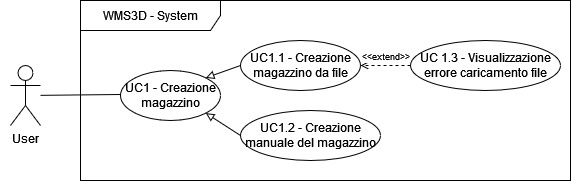
\includegraphics[width=0.8\textwidth]{UC_diagrams_1-10/UC1_sys.drawio.png}
    \caption{Diagramma UML UC1}
\end{figure}
\begin{itemize}
    \item \textbf{Attori:} User.
    \item \textbf{Pre-condizione:} L'applicazione è avviata e funzionante.
    \item \textbf{Post-condizione:} Il magazzino viene creato e potrà essere visualizzato.
    \item \textbf{Scenario Principale:}  L’utente accede al sistema e sceglie una modalità di costruzione o attraverso file [UC1.1] o manualmente [UC1.2]. I dati necessari sono poi inseriti correttamente dall'utente e il magazzino viene costruito.
    \item \textbf{Generalizzazioni:} Sono presenti due generalizzazioni: 
    \begin{itemize}
        \item UC1.1 - Creazione magazzino tramite file;
        \item UC1.2 - Creazione manuale del magazzino.
    \end{itemize}
    \item \textbf{Estensioni:} -
\end{itemize}


\subsubsection{UC1.1 - Creazione magazzino da file}
\begin{itemize}
    \item \textbf{Attori:} User.
    \item \textbf{Pre-condizione:} L'applicazione è avviata e funzionante e l'utente dispone di un file contenente tutti i dati di costruzione di un magazzino 3D.
    \item \textbf{Post-condizione:} I dati vengono caricati correttamente e il magazzino viene creato e potrà essere visualizzato.
    \item \textbf{Scenario Principale:}  L’utente accede al sistema e sceglie la modalità di costruzione attraverso file. Procede dunque al caricamento dei dati tramite file e il magazzino viene costruito.
    \item \textbf{Generalizzazioni:} -
    \item \textbf{Estensioni:} È presente una estensione:
    \begin{itemize}
        \item UC1.3 - Visualizzazione errore caricamento file.
    \end{itemize}
\end{itemize}


\subsubsection{UC1.2 - Creazione manuale del magazzino}
\begin{figure}[H]
    \centering
    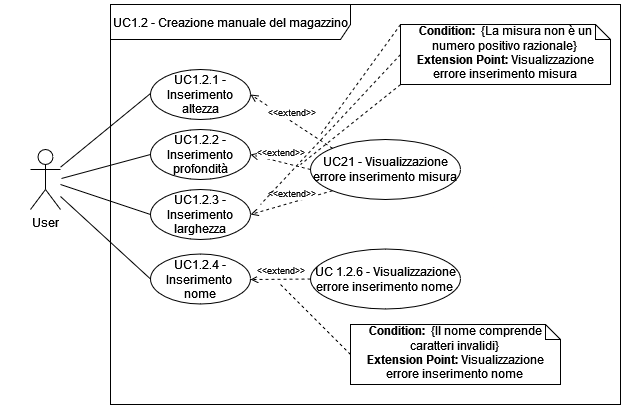
\includegraphics[width=0.8\textwidth]{UC_diagrams_1-10/UC1.2.drawio.png}
    \caption{Diagramma UML UC1.2}
\end{figure}
\begin{itemize}
    \item \textbf{Attori:} User.
    \item \textbf{Pre-condizione:} L'applicazione è avviata e funzionante e l'utente desidera creare un nuovo magazzino 3D.
    \item \textbf{Post-condizione:} Un nuovo magazzino vuoto viene creato e potrà essere visualizzato.
    \item \textbf{Scenario Principale:}  L’utente accede al sistema e sceglie la modalità di costruzione manuale. Inserisce i dati del magazzino, quali altezza [UC1.2.1], profondità [UC1.2.2], larghezza [UC1.2.3] e nome [UC1.2.4]), che vengono correttamente processati e il magazzino viene costruito.
    \item \textbf{Generalizzazioni:} -
    \item \textbf{Estensioni:} -
\end{itemize}


\paragraph{UC1.2.1 - Inserimento altezza}
\begin{itemize}
    \item \textbf{Attori:} User.
    \item \textbf{Pre-condizione:}  L'applicazione è avviata e funzionante e l'utente ha scelto di creare manualmente un nuovo magazzino 3D.
    \item \textbf{Post-condizione:} Viene inserita l'altezza per il nuovo magazzino.
    \item \textbf{Scenario Principale:}  L’utente inserisce l'altezza del magazzino da costruire.
    \item \textbf{Generalizzazioni:} -
    \item \textbf{Estensioni:} È presente una estensione:
    \begin{itemize}
        \item UC21 - Visualizzazione errore inserimento misura.
    \end{itemize}
\end{itemize}


\paragraph{UC1.2.2 - Inserimento profondità}
\begin{itemize}
    \item \textbf{Attori:} User.
    \item \textbf{Pre-condizione:}  L'applicazione è avviata e funzionante e l'utente ha scelto di creare manualmente un nuovo magazzino 3D.
    \item \textbf{Post-condizione:} Viene inserita la profondità per il nuovo magazzino.
    \item \textbf{Scenario Principale:}  L’utente inserisce la profondità del magazzino da costruire.
    \item \textbf{Generalizzazioni:} -
    \item \textbf{Estensioni:} È presente una estensione:
    \begin{itemize}
        \item UC21 - Visualizzazione errore inserimento misura.
    \end{itemize}
\end{itemize}


\paragraph{UC1.2.3 - Inserimento larghezza}
\begin{itemize}
    \item \textbf{Attori:} User.
    \item \textbf{Pre-condizione:}  L'applicazione è avviata e funzionante e l'utente ha scelto di creare manualmente un nuovo magazzino 3D.
    \item \textbf{Post-condizione:} Viene inserita la larghezza per il nuovo magazzino.
    \item \textbf{Scenario Principale:}  L’utente inserisce la larghezza del magazzino da costruire.
    \item \textbf{Generalizzazioni:} -
    \item \textbf{Estensioni:} È presente una estensione:
    \begin{itemize}
        \item UC21 - Visualizzazione errore inserimento misura.
    \end{itemize}
\end{itemize}


\paragraph{UC1.2.4 - Inserimento nome}
\begin{itemize}
    \item \textbf{Attori:} User.
    \item \textbf{Pre-condizione:}  L'applicazione è avviata e funzionante e l'utente ha scelto di creare manualmente un nuovo magazzino 3D.
    \item \textbf{Post-condizione:} Viene inserito il nome del nuovo magazzino.
    \item \textbf{Scenario Principale:}  L’utente inserisce il nome del magazzino da costruire.
    \item \textbf{Generalizzazioni:} -
    \item \textbf{Estensioni:} È presente una estensione:
    \begin{itemize}
        \item UC1.2.6 - Visualizzazione errore inserimento nome.
    \end{itemize}
\end{itemize}


\paragraph{UC1.2.6 - Visualizzazione errore inserimento nome}
\begin{itemize}
    \item \textbf{Attori:} User.
    \item \textbf{Pre-condizione:}  L'utente ha inserito come nome del magazzino un valore comprendente caratteri invalidi.
    \item \textbf{Post-condizione:} L'utente visualizza un messaggio d'errore e l'operazione fallisce.
    \item \textbf{Scenario Principale:}  L'utente visualizza un messaggio informativo sull'errore e ne conferma la ricezione. L'operazione, di conseguenza, fallisce.
    \item \textbf{Generalizzazioni:} -
    \item \textbf{Estensioni:} -
\end{itemize}


\subsubsection{UC1.3 - Visualizzazione errore caricamento file}
\begin{itemize}
    \item \textbf{Attori:} User.
    \item \textbf{Pre-condizione:} L'utente fornisce un file in un formato non supportato o con dati non validi.
    \item \textbf{Post-condizione:} L'utente visualizza un messaggio d'errore e l'operazione fallisce.
    \item \textbf{Scenario Principale:}  L'utente visualizza un messaggio informativo sull'errore e ne conferma la ricezione. L'operazione, di conseguenza, fallisce.
    \item \textbf{Generalizzazioni:} -
    \item \textbf{Estensioni:} -
\end{itemize}